\documentclass[11pt]{article}

\usepackage{graphicx}

\title{Understanding the Galois/Counter Mode (GCM) \large HW3 - CNS Sapienza}
\author{Matteo Salvino 1708108}
\date{21 November 2019}

\begin{document}
\maketitle
\section{Goal}
In this homework we are interested in to understand how \textit{Galois Counter Mode} works, in particular we will choose a specific symmetric encryption algorithm and compare this mode of operation with another one, in order to measure the encryption/decryption speed and ease of use. We want to underline that in this report we won't talk about the mechanisms behind  GCM because they will be explained in few slides attached to this report.
\section{Cipher Block Chaining vs Galois Counter Mode}
In order to setting up a comparison environment we chosen \textit{AES} with key length equal to 256 bits as symmetric encryption algorithm, \textit{Cipher Block Chaining} as first mode of operation and \textit{Galois Counter Mode} as the second one. Our environment will run on native Linux operating system, and will use OpenSSL to perform encryption and decryption processes. We wrote a small bash script in order to generate four files with different size (100KB, 1MB, 10MB and 100MB), then we pick three jpg images (small, medium and large) from internet to see how these two mode of operation behave when they are tested on text and binary files. In order to make several comparisons we wrote a bash script that runs 10 time the encryption and decryption process in order to take an average encryption/decryption speed measured in MB/s.\\\\Lets start with AES in CBC mode. Furthermore, we will report also the average speed ratio, because we though it is a good comparison measure. The results can be summarized in the following table :
\begin{center}
\begin{tabular}{| c | c | c | c |}
\hline
\multicolumn{4}{|c|}{AES-CBC} \\
\hline
File & Encryption (MB/s) & Decryption (MB/s) & Speed ratio\\
\hline
file01.txt & 4.94 & 5.39 & 0.9165 \\
\hline
file1.txt & 44.43 & 49.62 & 0.8954 \\
\hline
file10.txt & 222.32 & 281.70  & 0.7892 \\
\hline
file100.txt & 309.01 & 469.75 & 0.6578 \\
\hline
\end{tabular}
\end{center}
and seen in the plots below :
\begin{center}
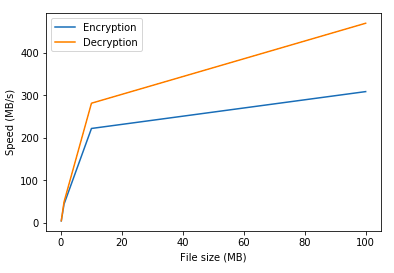
\includegraphics[scale=0.40]{./aes_cbc_speed_comparison.png}
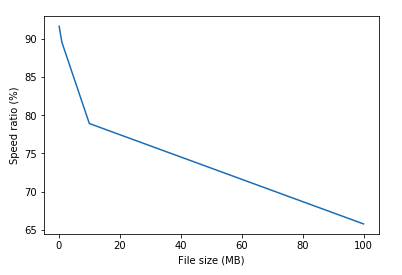
\includegraphics[scale=0.40]{./aes_cbc_speed_ratio.png}
\end{center}
Now, lets analyze how AES in CBC mode behave encrypting and decrypting binary files. In particular, the images in this experiment have dimension respectively 400KB, 2.6MB and 7MB. The results can be reported in the following table : 
\begin{center}
\begin{tabular}{| c | c | c | c |}
\hline
\multicolumn{4}{|c|}{AES-CBC} \\
\hline
File & Encryption (MB/s) & Decryption (MB/s) & Speed ratio\\
\hline
small.png & 16.92 & 17.14 & 0.9871 \\
\hline
medium.png & 90.05 & 101.55 & 0.8867 \\
\hline
large.png & 174.02 & 214.91  & 0.8097 \\
\hline
\end{tabular}
\end{center}
and seen in the plots below :
\begin{center}
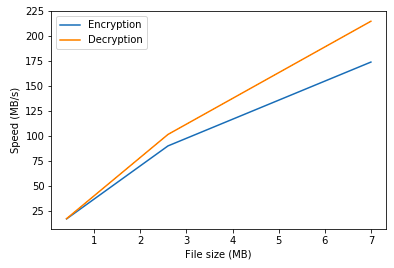
\includegraphics[scale=0.4]{./aes_cbc_speed_comparison_images.png}
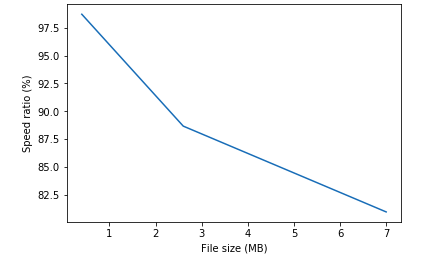
\includegraphics[scale=0.4]{./aes_cbc_speed_ratio_images.png}
\end{center}
Until now, we have seen that the encryption and decryption speed about AES in CBC mode, seems to grown with the size of the input file. Now, we want to analyze also AES in GCM to understand if it has better performance than AES-CBC or not. At the end of this report we will discuss also the ease of use of both modes. At the moment lets look how AES in GCM behave with input text file :
\begin{center}
\begin{tabular}{| c | c | c | c |}
\hline
\multicolumn{4}{|c|}{AES-GCM} \\
\hline
File & Encryption (MB/s) & Decryption (MB/s) & Speed ratio\\
\hline
file01.txt & 4.93 & 5.18 & 0.9517 \\
\hline
file1.txt & 44.60 & 48.52 & 0.9192 \\
\hline
file10.txt & 246.34 & 244.90  & 1.00 \\
\hline
file100.txt & 478.35 & 455.31  & 1.0506 \\
\hline
\end{tabular}
\end{center}
and shown in the following plots :
\begin{center}
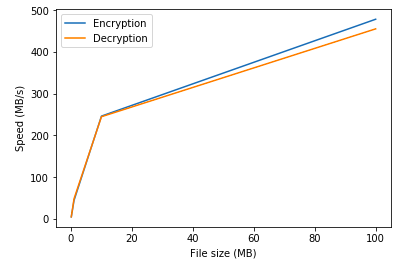
\includegraphics[scale=0.4]{./aes_gcm_speed_comparison.png}
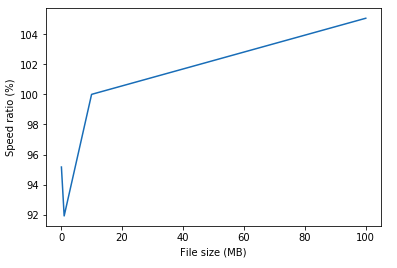
\includegraphics[scale=0.4]{./aes_gcm_speed_ratio.png}
\end{center}
Now, lets see how AES in GCM behaves with binary files :
\begin{center}
\begin{tabular}{| c | c | c | c |}
\hline
\multicolumn{4}{|c|}{AES-GCM} \\
\hline
File & Encryption (MB/s) & Decryption (MB/s) & Speed ratio\\
\hline
small.png & 15.79 & 16.61 & 0.9506 \\
\hline
medium.png & 94.66 & 98.19 & 0.9640 \\
\hline
large.png & 189.11 & 189.34  & 0.9987 \\
\hline
\end{tabular}
\end{center}
\begin{center}
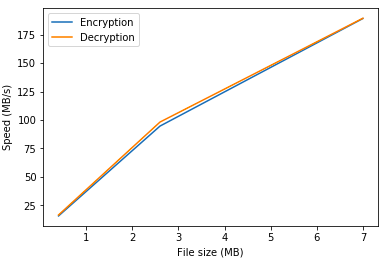
\includegraphics[scale=0.4]{./aes_gcm_speed_comparison_images.png}
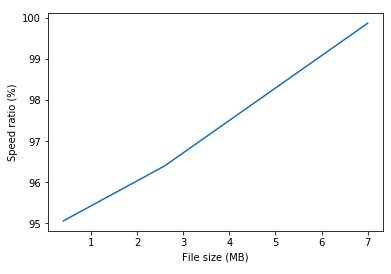
\includegraphics[scale=0.4]{./aes_gcm_speed_ratio_images.png}
\end{center}
\section{Results Comparison}
As we can see from the results, AES in CBC mode is faster in decryption process than encryption process, for the simply reason that the latter cannot be parallelized since each ciphertext block depends from the previous one, whereas in the decryption phase we have available all ciphertext blocks and thus we can parallelize it. Due to this facts as the input file size increases, the average speed ratio decreases. Passing to AES in GCM, we figure out that the trend is completely opposite. In this case both the encryption and decryption process are parallelizable, but as the input file size increases, the first one becomes faster than the second one, leading to an increasing average speed ratio.
\section{Conclusions}
Thus AES in CBC mode is slower than AES in GCM. Furthermore, the latter generate an authentication tag in order to provide both data integrity and data confidentiality. Naturally, each of these mode of operation has specific security requirement that must be respected in order to decreases the likely hood that your message could be revealed. In CBC if the size of plaintext isn't a multiple of cipher block size then the message must be padded, whereas in AES-GCM there isn't this necessity. Furthermore, in the first mode if a transmission error happen then the error is propagated to all successive blocks. In the second mode this doesn't happen, because each ciphertext block is treated as a single message. In the end, AES-GCM seems to be easier to use and more secure than AES-CBC.
\end{document}